\documentclass[10pt, openany]{book}

\usepackage[svgnames]{xcolor}
% ------------ pdf import per liberatoria e dichiarazione di conformita'
\usepackage{pdfpages}

% --------- math packages
% theorems
\usepackage{amsthm}
\usepackage{amsmath}
\usepackage{amssymb}
\usepackage{amsfonts}
\usepackage{upgreek} % uptau
\usepackage{siunitx}
\usepackage{caption}
\usepackage{subcaption}
\usepackage{stackrel}
\usepackage{mathtools} % norm
\usepackage[inline]{enumitem}
\usepackage{fancyhdr}
\usepackage{hyperref}
\usepackage{cleveref}
\usepackage{graphicx}
\usepackage{svg}
\usepackage{calc}
\usepackage{mdframed}
\usepackage{environ} % to declare scaletikzpicturetowidth with NewEnviron

% ------------ font related packages
% stuff for utf16
\usepackage{unicode-math-luatex}
\usepackage{unicode-math}
\usepackage{fontspec}
\usepackage{lmodern} % more font sizes

\setmathfont[mathrm=sym]{Latin Modern Math}

% ------------------ page layout
\usepackage{geometry}
\geometry{
	inner=37.125mm,
	outer=33.4125mm,
	top=37.125mm,
	bottom=37.125mm,
	heightrounded,
	marginparwidth=51pt,
	marginparsep=17pt,
	headsep=24pt,
}

% ------------- beautiful tables
\usepackage{booktabs}

% -------------- the bibliography
\usepackage[
	backend=biber,
	style=alphabetic,
	sorting=ynt
]{biblatex}

% ------------------- graphics
\usepackage{tikz}
\usepackage{pgfplots}
\usepackage{physics}
\usepackage{ifthen}
\usetikzlibrary{shadings}
\usetikzlibrary{calc}
\usetikzlibrary{arrows,arrows.meta} % Stealth arrows
\usetikzlibrary{angles,quotes} % for \draw pic (angle labels)
\usetikzlibrary{graphs,graphdrawing} % tree drawing for Owen Scrambling
\usegdlibrary{trees}
\tikzset{>=latex} % for LaTex arrow head

\makeatletter
\newsavebox{\measure@tikzpicture}
\NewEnviron{scaletikzpicturetowidth}[1]{%
	\def\tikz@width{#1}%
	\def\tikzscale{1}\begin{lrbox}{\measure@tikzpicture}%
	\BODY
	\end{lrbox}%
	\pgfmathparse{#1/\wd\measure@tikzpicture}%
	\edef\tikzscale{\pgfmathresult}%
	\BODY
}

\newsavebox\myboxA
\newsavebox\myboxB
\newlength\mylenA

\newcommand*\xoverline[2][0.75]{%
	\sbox{\myboxA}{$\m@th#2$}%
	\setbox\myboxB\null% Phantom box
	\ht\myboxB=\ht\myboxA%
	\dp\myboxB=\dp\myboxA%
	\wd\myboxB=#1\wd\myboxA% Scale phantom
	\sbox\myboxB{$\m@th\overline{\copy\myboxB}$}%  Overlined phantom
	\setlength\mylenA{\the\wd\myboxA}%   calc width diff
	\addtolength\mylenA{-\the\wd\myboxB}%
	\ifdim\wd\myboxB<\wd\myboxA%
	\rlap{\hskip 0.5\mylenA\usebox\myboxB}{\usebox\myboxA}%
	\else
	\hskip -0.5\mylenA\rlap{\usebox\myboxA}{\hskip 0.5\mylenA\usebox\myboxB}%
	\fi}
\makeatother

% -------------------------- code highlighting 
\usepackage[outputdir=intermediate]{minted}

% ------------------------- colors and other stuff for figures
% EM wavw
\colorlet{myblue}{black!40!blue}
\colorlet{myred}{black!40!red}
\colorlet{vcol}{green!50!black}
\colorlet{Ecol}{orange!90!black}
\colorlet{EVcol}{orange!80!black!60}
\colorlet{Bcol}{violet!90}

% EM spectrum
\colorlet{wavecol}{orange!35!black}
\colorlet{freqcol}{green!25!black}
\colorlet{enercol}{blue!35!black}
\pgfdeclareverticalshading{rainbow}{100bp}{
	color(0bp)=(red); color(25bp)=(red); color(35bp)=(yellow);
	color(45bp)=(green); color(55bp)=(cyan); color(65bp)=(blue);
	color(75bp)=(violet); color(100bp)=(violet)
}

% ------------------- units of measurements consistent style
\sisetup{
	detect-all,
	inter-unit-product=\ensuremath{{}\cdot{}},
  	separate-uncertainty=true,
  	uncertainty-separator={\,},
  	range-units=single,
  	per-mode=symbol,
  	exponent-product=\cdot,
  	output-decimal-marker={,},
}

% ----------------------------------- symbol definitions
% imaginary unit
\newcommand{\iu}{{i\mkern1mu}}

% ---------------- glossaries
\usepackage[toc]{glossaries}
\usepackage{monte-carlo-glossary}
\makeglossaries

% -------------------------- better management of larger projects
\usepackage{import}

% ----------------- stuff for customized title page
\usepackage{titling}
\usepackage{titlesec}

% -------------------------- tables
\usepackage{tabularx} % equal spacing
\usepackage{tabulary} % spacing proportional to content
\usepackage{xltabular} % multipage tabularx
\usepackage{multirow}

% left-justified text in tables, and allow newlines
\newcolumntype{Y}{>{\raggedright\arraybackslash}X}
\newcolumntype{U}{>{\raggedright\arraybackslash}c}

% bibliography declaration
\addbibresource{references.bib}

% default font times new roman
\renewcommand{\familydefault}{\rmdefault}

% definition environment
\newtheoremstyle{theoremdd}% name of the style to be used
	{\topsep}% measure of space to leave above the theorem. E.g.: 3pt
  	{\topsep}% measure of space to leave below the theorem. E.g.: 3pt
  	{}% name of font to use in the body of the theorem
  	{0pt}% measure of space to indent
  	{\bfseries}% name of head font
  	{. ---}% punctuation between head and body
  	{ }% space after theorem head; " " = normal interword space
  	{\thmname{#1}\thmnumber{ #2}\textnormal{\thmnote{ (#3)}}}
\theoremstyle{theoremdd}
\newtheorem{definitionS}{Def.}[section] % numbered by section
\newtheorem{definitionC}{Def.}[chapter] % numbered by chapter, to use when I need a def in beginning of chapter
\newtheorem{theoremS}{Th.}[section] % numbered by section

% shortcut to typeset code
\newcommand{\code}[1]{{\fontsize{10pt}{12pt}\fontfamily{qcr}\selectfont{#1}}}
\newfontfamily\codefont{DejaVu Sans}
\newcommand\tab[1][1cm]{\hspace*{#1}}
\newcommand{\littext}[1]{{\color{Rhodamine}{#1}}}
\newcommand{\hemi}[1]{\ensuremath{\mathfrak{H}^2(#1)}}
%\newcommand{\vector}[1]{\ensuremath{\mathbf{\overrightarrow{#1}}}}
\newcommand{\sha}{\ensuremath{\text{ш}}}

% footer setup using fancyhdr package
\setlength{\headheight}{15pt} % shut the warning up
\pagestyle{fancy}
\fancyfoot{} % to clear previous definitions of footer format
\fancyfoot[LE,RO]{\thepage}

\fancyhead{}
\fancyhead[LO]{\leftmark}
\fancyhead[RE]{\rightmark}

\newenvironment{altDescription}[1]
	{\begin{list}{}%
		{\renewcommand\makelabel[1]{\textsf{##1:}\hfil}%
			\settowidth\labelwidth{\makelabel{#1}}%
			\setlength\leftmargin{\labelwidth+\labelsep}}}
	{\end{list}}

\setmainfont{CharisSIL}
[
	Extension=.ttf,
	UprightFont=*-Regular,
	ItalicFont=*-Italic,
	BoldFont=*-Bold,
	BoldItalicFont=*-BoldItalic,
	Path=/usr/share/fonts/TTF/
]
\setmathfont{Latin Modern Math}
\setmathfont{XITSMath-Regular}
[
	Extension = .otf,
	BoldFont = XITSMath-Bold,
	Path=/usr/share/fonts/OTF/,
	range={"03F6,"0410-"044F}
]

%\setlength{\lineskip}{1.25pt}

% stuff for the title page of the document
\title{Metodi di Monte Carlo Applicati Alla Computer Grafica}
\author{Tanzi Alessio}
\newcommand{\professor}{Prof.ssa Marina Popolizio}
\date{Anno Accademico 2022/2023}

\begin{document}
	\begin{titlepage}
		\begin{center}
			\vspace*{1cm}
			{\Huge \bfseries \thetitle}\\ % title
			\vspace*{1cm}
			{\Large Tesi in Calcolo Numerico}
		\end{center}
		\vspace*{1cm}
		\begin{flushright}
			{\Large\bfseries Presentata da:\\\theauthor}
		\end{flushright}
		\begin{flushleft}
			{\Large\bfseries Relatore:\\\professor} 
		\end{flushleft}
		\vspace*{1cm}
		\begin{center}
			{\Large\thedate}
		\end{center}
	\end{titlepage}

	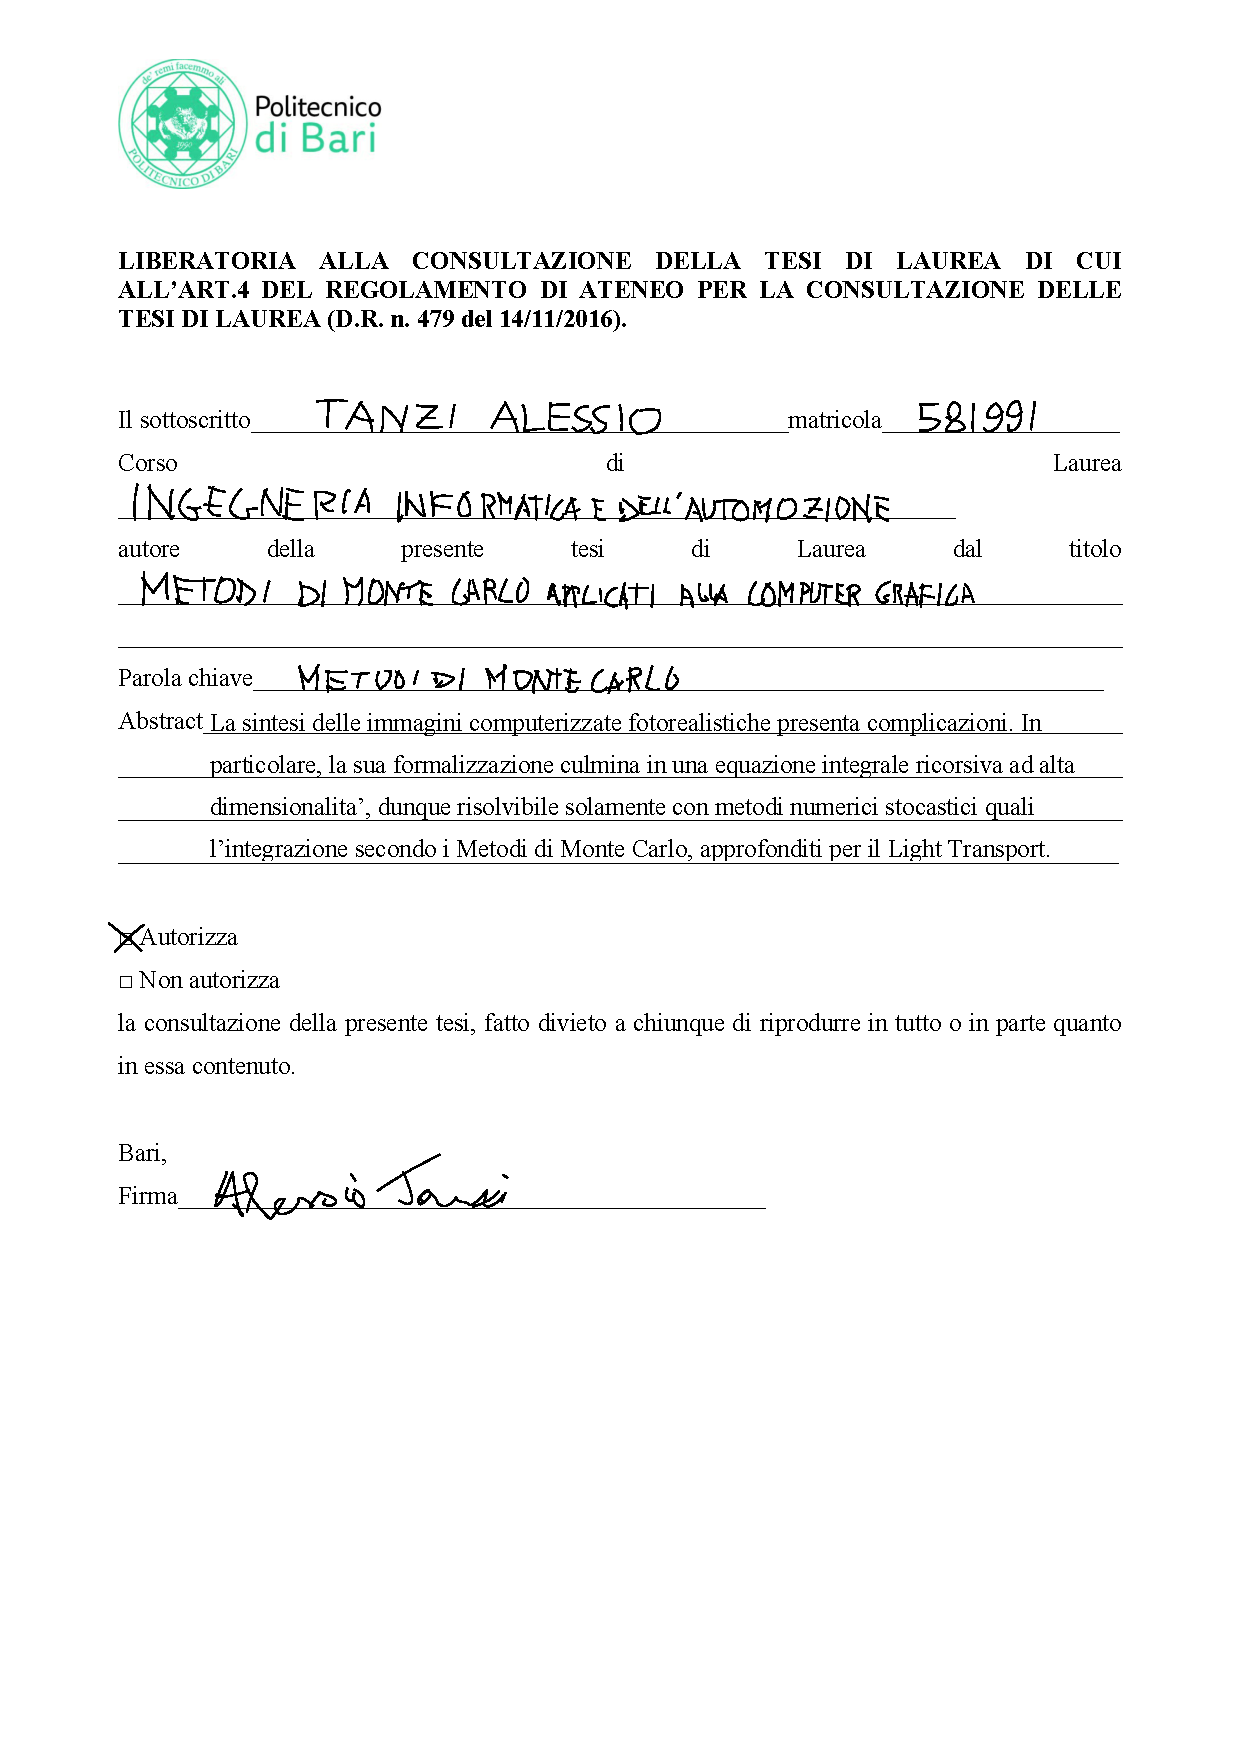
\includepdf{./LIBERATORIA_TESI.pdf}
	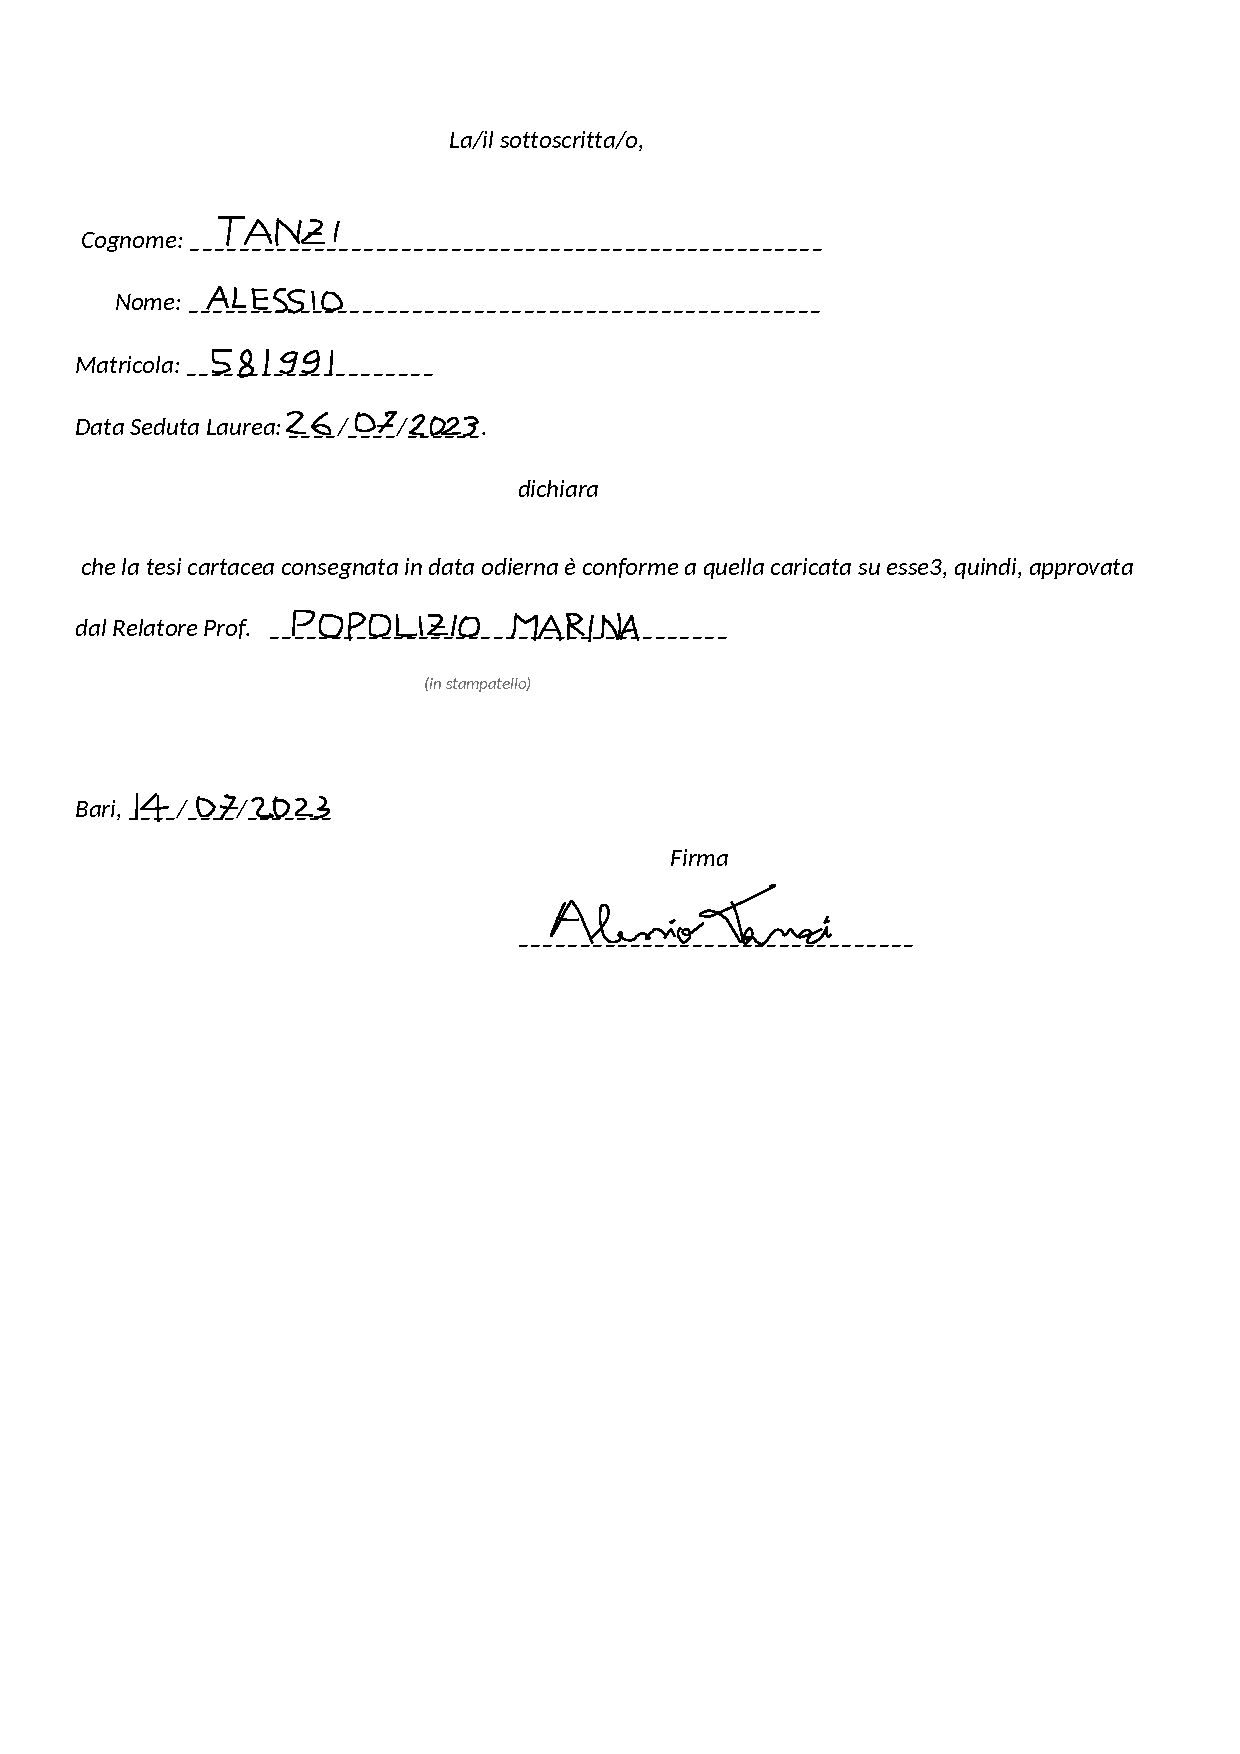
\includepdf{./Dichiarazione tesi conforme.pdf}

	\frontmatter
	\section*{Abstract}
	\begin{figure}[t]
		\centering
		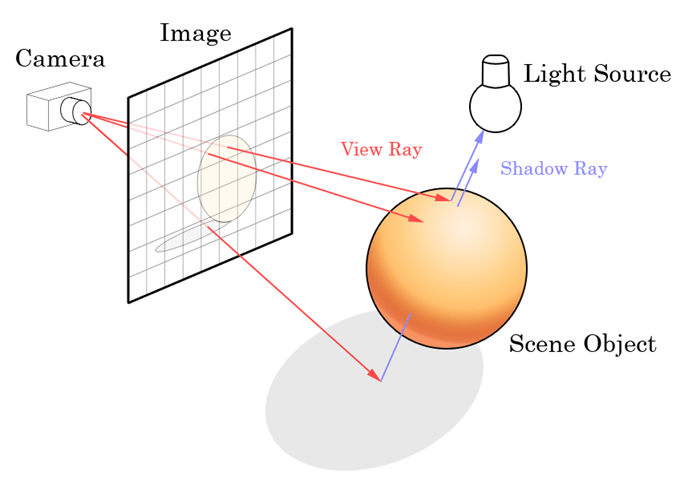
\includegraphics[width=0.6\linewidth]{./assets/intro_path_tracing_online_tech_tips.png}
		\caption{Illustrazione dell'algoritmo Path Tracing. L'obiettivo di questo documento \`e spiegare come i Metodi di Monte Carlo rendono 
			possibile la stima della funzione immagine $r_f(x,y)$}
		\label{intro:pathTracing}
	\end{figure}
	Nel seguente documento si presentano tutti i fondamenti matematici e scientifici al problema della sintesi di un immagine basata su fondamenti 
	fisici. A tal scopo, l'algoritmo proposto per la renderizzazione di scene tridimensionali \`e il \textit{Path Tracing}, il quale risolve il problema
	della \textit{Global Illumination}, cio\`e colorazione delle superfici contando illuminazione diretta ed indiretta.\par
	Immediatamente so presenta un problema per il calcolo di tale immagine (mostrata in Figura \ref{intro:pathTracing}): al fine di poter costituire 
	il risultato finale, l'\textit{Image Plane} \`e suddiviso a formare una griglia uniforme. In seguito, supponendo $r(x,y)$ funzione immagine,
	una data cella di area $A_{px}$ avr\`a colorazione pari all'integrale 
	\begin{equation}
		r_f(x,y)=\int_{A_{px}}r(x^\prime,y^\prime)\mathrm{d}A
	\end{equation}
	Immediatamente ci si rende conto che tale funzione non solo non \`e analiticamente integrabile, ma non \`e nota analiticamente. Infatti, $r(x,y)$
	pu\`o soltanto essere campionata, generando dei raggi con origine $\vec{o}$ pari alla posizione dell'osservatore, e direzione $\hat{\omega}$
	pari a $\mathmakebox{\tfrac{\vec{p}_i-\vec{o}}{\norm{\vec{p}_i-\vec{o}}}}$. Una volta campionato tale segnale bidimensionale, un filtro di
	ricostruzione $f(x,y)$ \`e utilizzato, mediante l'operazione di convoluzione $*$, per ottenere un'approssimazione della funzione immagine, filtrata,
	$r_f(x,y)$.
	\begin{equation}
		r_f(x,y)=\int_{A_{px}}f(x-x^\prime,y-y^\prime)r(x^\prime,y^\prime)\mathrm{d}A = (f*r)(x,y)
	\end{equation}
	Rimane per\`o il problema iniziale: per risolvere tale integrale, dovremmo estrarre $\infty$ campioni. Anche se ci\`o fosse possibile, l'integrale
	ottenuto non sarebbe risolvibile analiticamente. Tale espressione si presta alla risoluzione mediante i Metodi di Monte Carlo, del quale si 
	riporta qui lo stimatore pi\`u semplice
	\begin{equation}
		r_f(x,y)\approx\frac{\norm{A_{px}}}{n}\sum_{i=1}^{n}f(x-x_i,y-y_i)r(x_i,y_i)
	\end{equation}
	Si sposta l'attenzione allora al calcolo di ciascun campione: il suddetto raggio \`e propagato per la scena, finch\`e non interseca una superficie.
	Dunque, il compito adesso \`e quello di calcolare il colore che tale superficie emette. In quanto il concetto di colore \`e strettamente legato 
	alla percezione umana, tale computazione vede come grandezza utilizzata la \textit{Radianza Spettrale}, potenza uscente o incidente in un punto di 
	una superficie, da/a una data direzione. Tale grandezza \`e opportunamente campionata in punti equispaziati dello spettro visibile.\par 
	Come illustrato nei capitoli seguenti, l'equazione che determina la radianza spettrale uscente \`e l'\textit{Equazione del Rendering}
	\begin{equation}
		L_o(\vec{p},\hat{\omega}_o,\hat{\omega}_i)=L_e(\vec{p},\hat{\omega}_o)+%
			\int_{\mathcal{S}^2}f_r(\vec{p},\hat{\omega}_o,\hat{\omega}_i)L_i(\vec{p},\hat{\omega}_i)|\langle\hat{n},\hat{\omega}_i\rangle|
				\mathrm{d}\hat{\omega}_i
	\end{equation}
	Ovviamente, tale integrale presenta le stesse problematiche dell'equazione per pixel filtering, dunque va anch'esso risolto con il metodo di 
	Monte Carlo. Si noti per\`o, che tale espressione \`e ben pi\`u complicata da risolvere, e non solo perch\`e \`e ricorsiva.
	La funzione integranda presenta pi\`u fattori, altamente variabili, di termini fisici complessi, ed infatti la spiegazione di ciascuno 
	dei termini coinvolti e tattiche di campionamento per la funzione integranda sono oggetto di ben tre capitoli.\par
	Nelle pagine a seguire si propone di introdurre i Metodi di Monte Carlo, dimostrando la loro grande potenzialit\`a nella risoluzione del problema 
	presentato, fino a formulare la strategia completa dell'algoritmo di Path Tracing.

	\section*{Acknowledgements}
	Vorrei ringraziale la Prof.ssa Marina Popolizio che ha acceso in me la passione per il calcolo numerico e permesso di dedicarmici spostando anche 
	l'attenzione sulla grafica computerizzata, oggetto della mia curiosit\`a negli ultimi tempi. Inoltre, ringrazio la mia famiglia per avermi fornito
	coraggio e supporto per tutto il mio percorso.\par
	Spendo le ultime parole di questa introduzione per sottolineare quanto affascinante sia la Computer Grafica, quanto complicata. Di seguito, \`e 
	indicato il link per il codice relativo alla implementazione dei concetti qui spiegati:\\
	\href{https://github.com/alexoz12v2/monteCarlo}{https://github.com/alexoz12v2/monteCarlo}

	\tableofcontents

	\mainmatter
	\part{Introduzione ai Metodi di Monte Carlo}
	\import{chapters/}{chapter-part2-2-sampling-montecarlo.tex}
	\import{chapters/}{chapter-part2-1-quasirandom-gen.tex}
	\import{chapters/}{chapter-part3-1-light-transportintro.tex}

	\part{Fondamenti Fisici}
	\import{chapters/}{chapter-part1-1-electromagnetic-radiometry.tex}
	\import{chapters/}{chapter-part1-2-color-camera.tex}
	\import{chapters/}{chapter-part1-3-light-surface.tex}

	\part{Appendici}
	\appendix
	%\import{chapters/}{chapter-Appendix-A-prob-stat.tex}
	%\import{chapters/}{chapter-Appendix-B-geo-alg.tex}
	\import{chapters/}{chapter-Appendix-C-random-num.tex}
	\import{chapters/}{chapter-Appendix-D-vulkan-code.tex}
	%\import{chapters/}{chapter-Appendix-E-materials-impldetails.tex}

	\backmatter
	% Add bibliography to TOC
	\addcontentsline{toc}{chapter}{\bibname}
	\printbibliography

	\printglossaries
\end{document}

